% Template: http://www.acm.org/sigs/publications/proceedings-templates#aL2 
% 
\documentclass{icn/sig-alternate-2012} % {proc}

\usepackage{amsmath}    % need for subequations
\usepackage{graphicx}   % need for figures
\usepackage{verbatim}   % useful for program listings
\usepackage{color}      % use if color is used in text
\usepackage{subfigure}  % use for side-by-side figures
\usepackage{hyperref}   % use for hypertext links, including those to external documents and URLs
\usepackage{url}
\usepackage{multicol}
\usepackage{textcomp}
%\usepackage{caption}  %% supported in class
\usepackage{algorithm}
\usepackage{algpseudocode}
\usepackage{enumitem}

%\usepackage{authblk}  %% supported in class
% \usepackage{float}
% \newfloat{algorithm}{t}{lop}

\newcommand{\ndnrtcName}{NDN-RTC} % {\emph{ndnrtc}}
\newcommand{\ndnconName}{NdnCon}

%% Shrink lists - http://tex.stackexchange.com/questions/43743/how-to-reduce-line-space-leading-within-an-enumerate-environment 
\setenumerate{itemsep=-0.5ex,topsep=1ex, leftmargin=*}
\setitemize{itemsep=-0.5ex,topsep=1ex, leftmargin=*}



\title{\ndnrtcName{}: Real-time videoconferencing\\ over Named Data Networking}

\numberofauthors{2}
\author{
\alignauthor Peter Gusev\\
       \affaddr{UCLA REMAP}\\
       \email{peter@remap.ucla.edu}
\alignauthor Jeff Burke\\
       \affaddr{UCLA REMAP}\\
       \email{jburke@remap.ucla.edu}
}

\begin{document}

\maketitle

%************************************************
\abstract
\ndnrtcName{} is a real-time videoconferencing library using the Named Data Networking (NDN) future internet architecture. It was designed to provide a similar end-user experience to Skype or Google Hangouts, while taking advantage of the NDN architecture's data naming, signing, caching, and request aggregation. It demonstrates low-latency communication of HD video on NDN without direct producer-consumer coordination, enabling scaling to many consumers through the network architecture's intrinsic caching and request aggregation. Internally, it employs widely-used open source components, including the WebRTC library, VP9 codec, and OpenFEC (forward error correction). This paper presents the design, implementation in C++, and testing of \ndnrtcName{} on the NDN testbed using a graphical conferencing application implemented using the library.

%************************************************
\section{Introduction}
% About NDN from the standpoint of content distribution.
Named Data Networking (NDN) is a future internet architecture that shifts from the current internet's host-centered paradigm towards data-centered communication.~\cite{ndntechreport} In NDN, every chunk of data has a hierarchical name (often human-readable) which is used by routers to satisfy data requests called "interests". This data is also cached by a router and used to answer similar requests in the future. Initrinsic caching ability of NDN can be leveraged by content distribution applications and halp to offload data publishers significantly in multi-peer scenarios.

% About current low-latency applications and multi-party conferences.
Low-latency audio/video conferencing applications often require establishing direct peer-to-peer communication channels for the best user experience and face implementation challenges and inefficiencies related to connection-based approach currently used in most IP conferencing solutions. For example, consider the inefficiency of delivering duplicated media streams for other nine people participating in the same ten-party conference.

% About this project and what it does
\ndnrtcName{} is designed and implemented to further develop and explore NDN's potential for scalable low-latency audio/video conferencing. \ndnrtcName{} provides basic functionality for publishing audio/video streams and fetching any streams being published which can be leveraged by desktop or web applications for establishing multi-party conferences. While NDN gives scalability adavantages, \ndnrtcName{} ensures low-latency communication and that the data being fetched is the most recent currently available on the network. \ndnrtcName{} is a C++ library which is built atop WebRTC library, incorporating existing audio pipeline, including echo cancellation and existing video codec (VP9).

The rest of the paper is organized as follows. Section \ref{sec:bg} covers background and prior work. Section \ref{sec:goals} lists main goals of this project. Section \ref{sec:arch} describes architecture of the library, designed namespace, data structures and algorithms used. Section \ref{sec:imp} discusses implementation details. Section \ref{sec:eval} evaluates main outcomes of this project. Section \ref{sec:future} addresses future work and existing issues. Finally, Section \ref{ref:conclusion} concludes the paper.

%************************************************
\section{Background and prior work}
\label{sec:bg}
To authors' knowledge, \ndnrtcName{} is one of the few applications with perceptual real-time requirements tested on Information Centric Networking platform over a multi-hop testbed. 

A non-real time video-streaming software solution called NDNVideo \cite{ndnvideo} had successfully been tested and deployed on NDN network and prooved its' high scalability. The project focused on developing random-access and live video for location-based and mixed reality applications. Another conferencing application, however audio-only, was developed in \cite{act-tool}. It leveraged use of Mumble VoIP software but used NDN as a transport. Some initial effort for conference and user discovery is made in this work as well. This work suggests that building on an existing, resilient platform is the best way to generate a usable application. Therefore, \ndnrtcName{} was chosen to be built on top of WebRTC library in order to utilize its' audio-processing capabilities, video codecs and potentially give an opportunity for easier integration with the supported web-browsers.

% cite DASH over NDN 
% cite tech report from lixia's group (Ilya)
% cite any others? 

%************************************************
\section{Design Objectives}
\label{sec:goals}
The NDN project team uses application-driven research to explore the affordances of NDN for modern applications and refine the architecture itself.  Initial goals of the \ndnrtcName{} project are to explore low-latency audio/video communication over NDN and to provide a multi-party conferencing application which can be used by NDN project team members across existing NDN testbed. It can be also used as a traffic generator application for future researches in NDN routing algorithms, congestion control and general testing of the network architecture ideas.
\begin{itemize}
\item \textbf{Low-latency audio/video communication.} Library should be capable to maintain similar low-latency (150-300ms)  communication for audio and video as in dirver applications like Skype, WebEX, Goolg Hangouts.

\item \textbf{Multi-party conferencing.} Publishing and fetching several media streams simultaneously should not require significant computational resources from the user and should maintain the same latency as in one-to-one conferencing case.

\item \textbf{Passive consumer \& cacheability.} There should be no explicit negotiation or any coordination between active conference members as it may limit scalability and flexibility of use. Data should be cacheable for multiple consumers capable of decrypting it. 

\item \textbf{Data verification.} Library should provide content verification using existing NDN signature capabilities. 

\item \textbf{Encryption-based access control.}   (Not implemented in this version.)
\end{itemize} 

%************************************************
\section{Application Architecture}
\label{sec:arch}

\begin{figure}[t!]
\centering
\subfigure[Producer]{\label{fig:producer}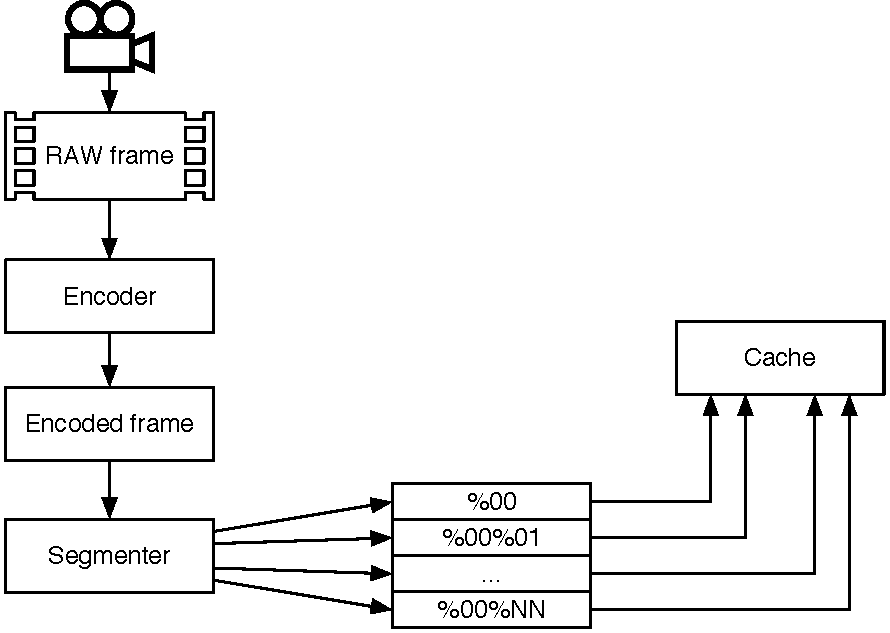
\includegraphics[width=0.4\textwidth]{producer}}\qquad
\subfigure[Consumer]{\label{fig:consumer}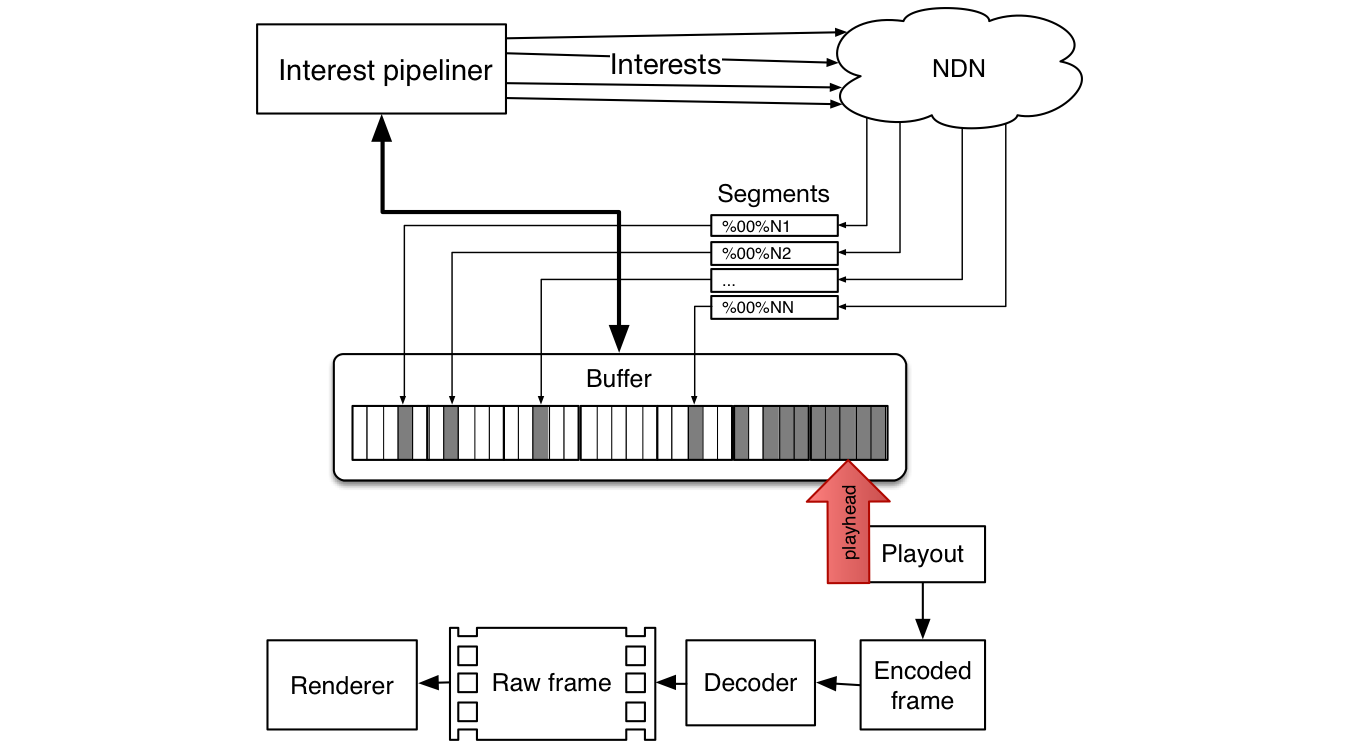
\includegraphics[width=0.4\textwidth]{consumer}}
\caption{\ndnrtcName{} producer and consumer operation.}
\end{figure}



There are two main roles defined in \ndnrtcName{}: producer and consumer. In presence of NDN network the paradigm of real-time communication shifts from the push-based (when producer writes data to the socket and consumer reads it as fast as possible) to the pull-based (producer publishes data on the network with his own pace, while consumer has to request the data he needs and manage incoming data segments).

% Redundant figure
%
%\begin{figure}[t!]
%\centering
%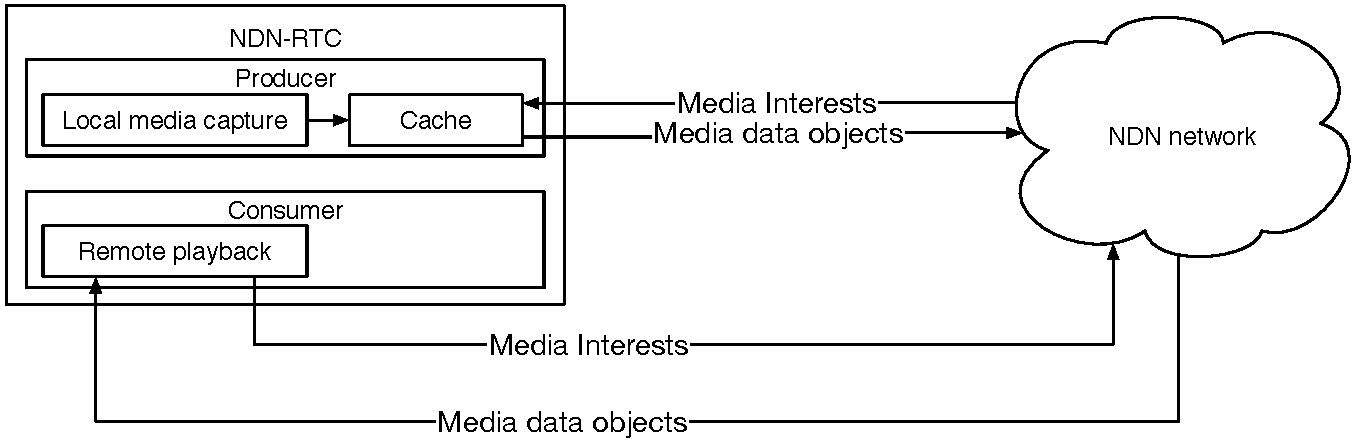
\includegraphics[width=0.5\textwidth]{architecture}
%\caption{RTC over NDN}
%\label{fig:arc}
%\end{figure}

Figure \ref{fig:arc} presents top-level overview of how \ndnrtcName{} works. Local media capture and Cache belong to the producer part of the \ndnrtcName{}. Media is stored in the cache which provides access to the data for all incoming interests. Remote playback represents consumer: it issues interests, prepares received media (assembles video frames from segments and re-orders them) and plays it back.

\subsection{Producer}
The producer's main task is to acquire video and audio data from media inputs, encode it, pack into network packets and store them in the cache for incoming Interests – in this way, complexity shifts to the consumer, and scaling is supported by the network.

In case of video streaming, producer uses video encoding in order to reduce size of the frames. There are two types of encoded frames: \textit{Key} and \textit{Delta}. Key frames contain the most of the video information and don't depend on any previous frames to be decoded. Whereas Delta frames are dependent on all previous frames received after the last Key frame and can't be decoded without significant visual artifacts if any of those frames are missing.

Encoded frames vary in size, but average bitrate stays the same. For example, the average sizes of frames for 1000 kbps stream using VP8/VP9: Key frames are $\approx$ 30KB, delta frames are $\approx$ 3-7KB.
Therefore, depending on the underlying internet protocol used (IP in the existing NDN testbed), producer may need to segment encoded frames into a smaller chunks and provide clear naming conventions for consumer to fetch them.




%************************************************
\subsection{Namespace}

As there is no direct consumer-produder communication, it is producer's job to provide as much supportive information as possible so that consumer is able to use this information in order to achieve her goals. There are several kinds of data producer can publish and these kinds should be reflected in the namespace:
media data (segmented video frames and bundled audio samples), error correction data, and metadata. 

%Besides that, the namespace should also reflect data specialization hierarchy - from general concepts in the root to more specialized entities towards the leaves. 

\subsubsection{Media} 

\ndnrtcName{} producer uses a concept of \textit{media stream} for describing published media. Media stream represents a flow of raw media packets (video frames or audio samples) coming from an input device. Streams usually derive names from their input devices. It is quite natural for a producer to publish several media streams simultaneously, if she has more than one device to publish media from (for instance, publish video from camera, audio from microphone and another video stream for sharing computer screen). As all raw data should be encoded, the next level in the name hierarchy represents different encoder instances called \textit{media threads}. Thus, media threads allow producer to provide same media stream in several copies, for instance in low, medium and high quality for video, so that consumer can have a chance to choose media thread more suitable for the current network conditions.

%\begin{figure}[t!]
%\centering
%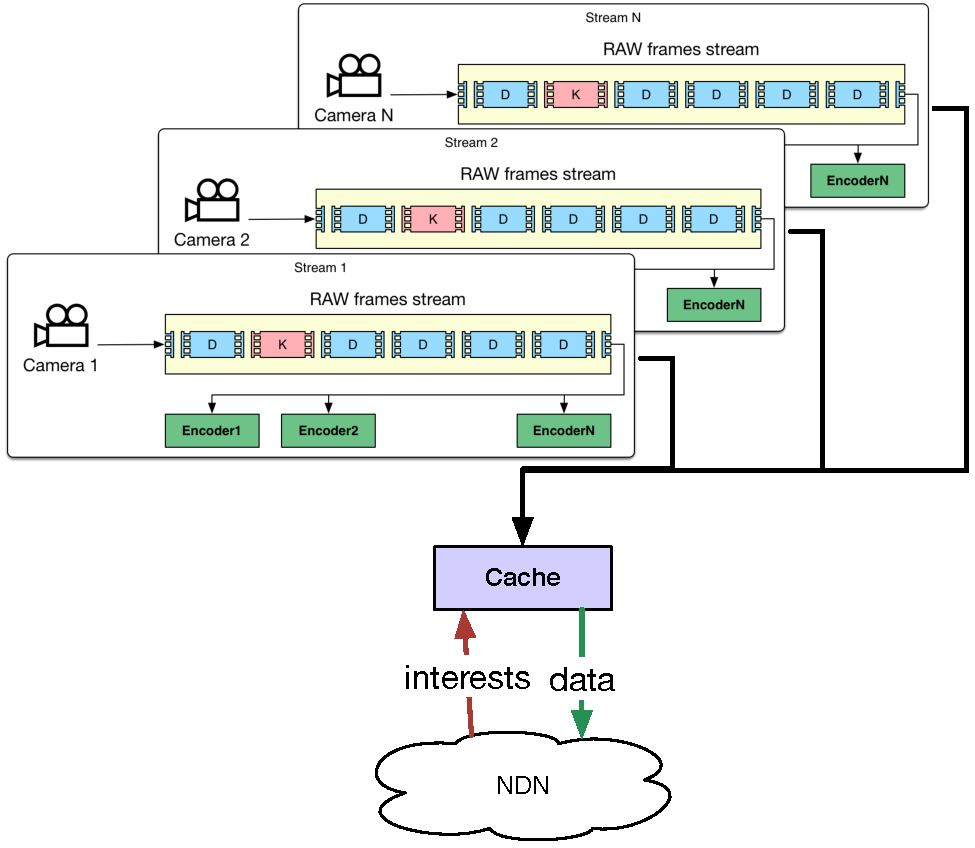
\includegraphics[width=0.5\textwidth]{streams-hierarchy}
%\caption{\ndnrtcName{} media streams hierarchy}
%\label{fig:stream-hierarchy}
%\end{figure}

\ndnrtcName{} does not use any specific media container format for delivering its media to consumers. Instead, encoded media packets are segmented if needed and published under distinctive hierarchical names. Video frames are separated into two domains as per frame type: \textit{delta} and \textit{key} and numbered sequentially and independently. Both sequence numbers for delta and key frames start from 0. Next level specializes data type - it can be either media data or parity. Parity data, if producer opts to publish it, can be used by consumer to recover frames that miss one or more segments. The topmost level of the namespace defines individual data segments. These segments are also numbered suquentially and segment numbers conform to NDN naming conventions \cite{ndn_naming}.

There are some differences in case of the audio streams. First, there are no key frames, therefore all the audio packets are published under the \textit{delta} namespace. Second, audio samples are significantly smaller than video frames and do not require to be segmented. In practice, it appears that multiple audio samples can be bundled into one data segment. Therefore, instead of segmenting audio packets, they are bundled together until the size of one data segment is reached and published only after that.

Consumers need to know producer's streams structure in order to fetch data successfully. In order to save consumer from traversing actual producer's name tree, which can be time-consuming and unreliable, producer publishes meta information about her current streams under \textit{session info} component. Thus, consumers can retrieve up-to-date information about the producer's state.

\begin{figure}[t!]
\centering
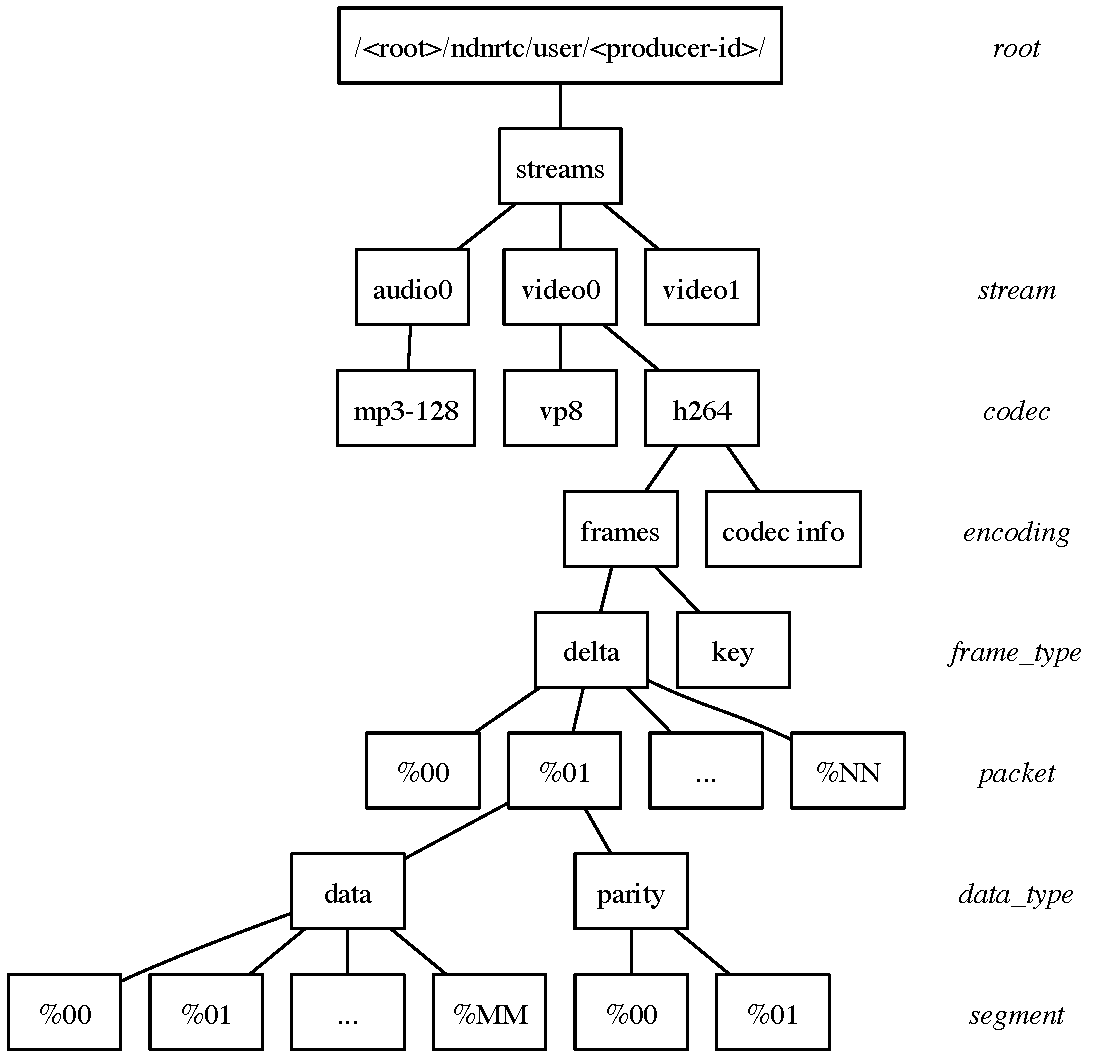
\includegraphics[width=0.45\textwidth]{namespace}
\caption{\ndnrtcName{} namespace}
\label{fig:namespace}
\end{figure}

\subsubsection{Metadata} 

Besides naming data objects, data names can be appended by some additional media-level meta information which can be utlilized by consumers regardless of which frame segment was received first. Three components are added at the end of every data segment name:
\small\begin{equation}
.../\textbf{segment\#}/\textbf{playback\#}/\textbf{paired\_seq\#}/\textbf{num\_parity} \nonumber
\end{equation}\normalsize
\begin{itemize}[label={}]
\item \textit{playback\#} - absolute playback number for current frame; this is different from the \textit{frame\#} which is a sequential number for the frame in its' domain (i.e. Key or Delta);
\item \textit{paired\_seq\#} - sequential number of the corresponding frame from other domain (i.e. for delta frames, it is sequential number of the corresponding key frame which is required for decoding);
\item \textit{num\_parity} - number of parity segments for this particular frame.
\end{itemize}

The pull-based nature of NDN and our experimental application's deliberate avoidance of explicit consumer-producer synchronization (allowing publisher-independent scaling) have shown the importance of providing sufficient meta information on producer side. Such information - which could include interests' nonce values, interests' arrival timestamps and data generation delays - if added to the returned data segment may help consumers evaluate relevant network performance, detect congestion and assess whether incoming data is likely to be stale (delayed beyond the path delay). Further, keeping historical data on consumer side may help perform better interest pipelining in the future. For instance, providing the average number of segments per frame type helps consumer make better guesses on the number of required initial interests to fetch upcoming frames, thus keeping frame fetching cycles minimal.


%************************************************
\subsection{Data objects}
Producer generates signed data objects from input media streams and places them in cache instantly. Incoming interests retrieve data from cache, if it is present, or forwarded further to the producer, if the requested data has not been produced yet. In such cases, producer maintains a pending interests table (PIT), which is checked every time new data object is generated. If an interest for newly generated data object exists in the PIT, it gets answered and PIT entry is erased.

\subsubsection{Media stream}
%% TODO: What's the media payload? 

\begin{figure}[t!]
\centering

\subfigure[video frame segmentation]{\label{fig:segment}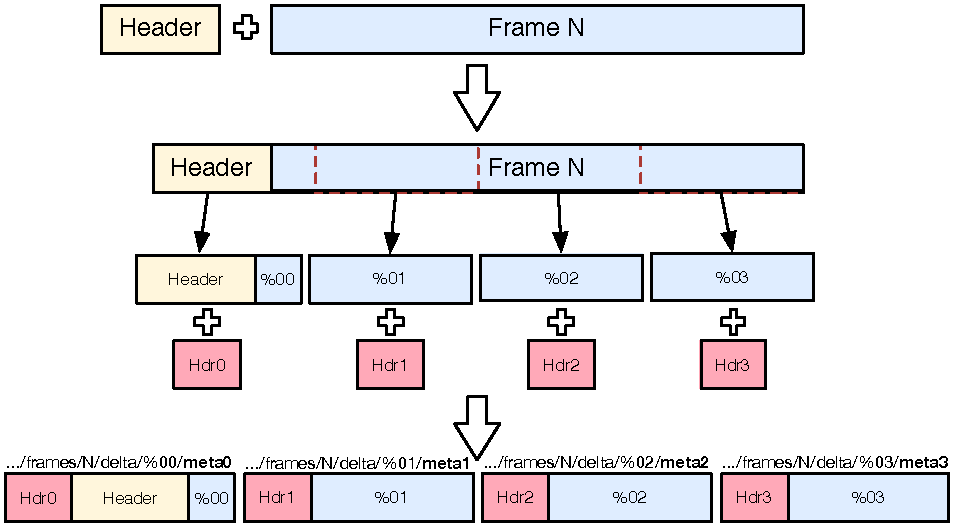
\includegraphics[width=0.5\textwidth]{segmentation}}
\subfigure[audio samples bundling]{\label{fig:audio-bundling}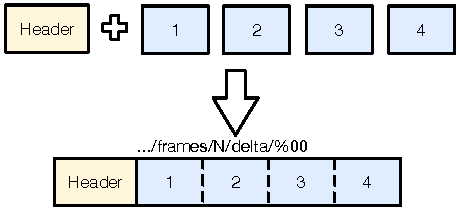
\includegraphics[width=0.3\textwidth]{audio-bundling}}

\caption{Segmentation and bundling}

\end{figure}

\subsubsection{Metadata}

Besides actual stream data, data objects contain some amount of meta information which is prepended during frames segmenting (see Figure \ref{fig:segment}). There are two types of headers: \textit{Frame header} and \textit{Segment header}. Frame header is prepended to segment \#0 of each individual video frame and contains media-specific information (such as size of a frame), timestamp, current rate and unix timestamp, which can be used for calculating actual delay between NTP-synchronized producer and consumers (see Figure \ref{fig:data-struct}). Segment header is prepended to every segment of a frame. It carries network-level information which can be used by consumer for making certain assumptions about current network conditions and origin of the data objects received:
\begin{itemize} [label={}]

\item \textit{Interest arrival timestamp.} Timestamp of the interest arrival. Monitoring this value and interest expression timestamps over time may give consumer a clue about how long does it take for interests to reach producer. This value is only valid when nonce value belongs to one of the consumer's interests.

\item \textit{Generation delay.} Time interval in milliseconds between interest arrival and segment publishing. Consumer can use this value to her advantage in order to control the number of outstanding interests. This value is only valid when nonce value belongs to one of the consumer's interests.

\item \textit{Interest nonce.} Nonce value of the interest which requested this particular segment. There are three meaningful cases:  1) \textit{value belongs to the interest issued previously} - consumer received non-cached data requested by interest issued previously; 2) \textit{value is non-zero, but doesn't belong to any of the previously issued interests} - consumer received data requested by some other consumer; data may be cached; 3) \textit{value is zero} - consumer received data which was cached on producer side and never requested by anyone before.

\end{itemize}

\begin{figure}[t!]
\centering
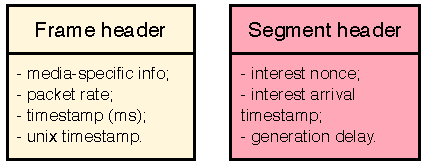
\includegraphics[width=0.3\textwidth]{data-struct}
\vspace{-4pt}
\caption{Frame and segment headers}
\label{fig:data-struct}
\end{figure}

Audio samples are not prepended by any segment header, however the whole audio bundle is prepended by the same frame header (see Figure \ref{fig:audio-bundling}).

%************************************************
\subsection{Consumer}

The Consumer implements more sophisticated algorithms to achieve following goals:
\begin{itemize}
\item ensure fetching the latest data available in the network; 
\item choose appropriate media stream bandwiths provided by a producer by monitoring network conditions;
\item playback fetched media in correct order;
\item handle network latency and packet drops.
\end{itemize}

Consumer takes into account that media packets are presented by separate segments in the network. Therefore, consumer implements mechanisms of interest pipelining and frame buffering (see Figure \ref{fig:consumer}). Interest pipeliner issues interests for individual segments and is controlled by some higher-level logic which achieves one out of four consumer's goals - ensures that only the latest data is fetched. Packets re-ordering, drops and latency fluctuations absorbtion are attained by the frame buffer which introduces buffering delay and re-arranges received frames in the playback order.



%************************************************
\subsubsection{Frame fetching}

Consumer doesn't know the total number of segments beforehand, unless the very first segment is fetched - in this case, consumer can retrieve metadata from the received segment and get total number of segments for the current frame. 
Therefore, at first attempt, consumer tries to make a "best guess" in the number of segments she needs to fetch by issuing $M$ interests (see Figure \ref{fig:pull}). If interests arrive too early, they will be added to the producer's PIT and stay there for some amount of time $d_{gen}$ called \texttt{generation delay}. Once encoded frame is segmented into $N$ segments, they are published and if $N\geq M$, interests $0 - M$ are answered with the data  which travels back to consumer. Upon receiving first data segment, consumer determines the total number of segments for the current frame and issues $N - M$ more interests for the missing segments if any. These segments will be satisfied by data with no generation delay (as the frame has been published already by producer). The time interval between receiving very first segment and until the frame is fully assembled is represented by $d_{asm}$ and called \texttt{assembling time}.

\begin{figure}[t!]
\centering
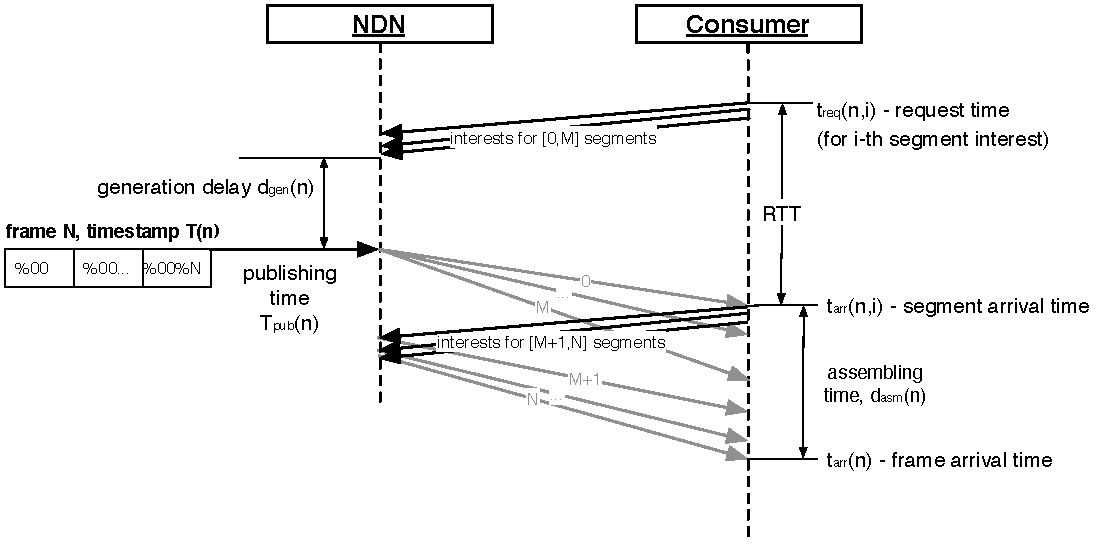
\includegraphics[width=0.5\textwidth]{frame-fetch}
\vspace{-18pt}
\caption{Fetching frame}
\label{fig:pull}
\end{figure}

It is needlesss to say, that additional round-trips for requesting missing data segments increase overall frame assembling time and chances that the frame will be incomplete by the time it should be played back. This problem could have been avoided if consumer could make a better guesses in the number of initial interests. Therefore, the following considerations were introduced in later versions of the library:
\begin{itemize}
\item consumer should know what type of frame she is going to fetch (as average number of segments varies greatly for different frame types);
\item consumer should track average number of segments per frame type.
\end{itemize}

The first consideration was implemented by introducing separate namespaces for key and delta frames. The second consideration helps consumer do better at guessing the number of initial interests.

\subsubsection{Buffering}

% Buffer:
% - re-ordering
% - added latency to mitigate network delays
% - extended defition:
% 	- pending frames
% 	- assembling frames
% - buffer-based retransmissions

As in traditional streaming applications, consumer uses frame buffering in order to tackle out-of-order data arrivals and network delay deviations. Consumer-side jitter buffer is also used as a place for assembling frames by segments. However, the definition of jitter buffer is extended for NDN networks. In traditional push-based approach, buffer can not contain empty frame slots - they are allocated/reserved only when data arrives. Pull-based paradigm requires consumer to request data explicitly. Therefore, after expressing interest consumer "knows" that new data is coming and a frame slot should be reserved in the buffer. Practically, this means, that there will always be some number of empty reserved slots in the buffer. Thus, jitter buffer's size have two measurements:
\begin{itemize}[label={}]
\item \textit{playback size} - playback duration of all complete ordered frames by the moment;
\item \textit{estimated size} = \textit{playback size} + \textit{number of reserved slots} $\times$ 1/\textit{producer rate}
\end{itemize}

The difference between estimated size and playback size ($RTT^{\prime}$) can't be smaller than the current average RTT value. In fact, keeping this value at a minimum indicates that consumer receives the most recent data with the minimal amount of outstanding interests. Monitoring this value over time may help consumer to get a clue on her "sync" status with the producer. For example, consumer may use it during fetching process as will be discussed in the next section. 

\subsubsection{Interest expression control}

The key challenge in a consumer-driven model for videoconferencing is to \emph{ensure the consumer gets the latest data in a caching network}, without resorting to direct producer-consumer communication that would limit scaling. To get fresh data, which can be cached but should not be the newest available for the consumer's path,  the consumer cannot rely only on using such flags as \textit{AnswerOriginKind} and \textit{RightMostChild}. The high frequency nature of streaming data makes no guarantees that the data satisfying those flags received by a consumer will be the most recent one. Instead, it is necessary to use other indicators to ensure that the network supplies up-to-date stream data. The basic solution is to leverage the known segment publishing rate and assume, under normal operation, that a series of old, cached samples, can be retrieved more quickly than new data. The inter-arrival delays ($D_{arr}$) of the most recent samples follow the publishers' generation pattern but cached data will follow interest expression temporal pattern. Therefore, by monitoring inter-arrival delays of consequtive media samples, consumers can make educated assumptions about data freshness (see Figure \ref{fig:inter-arrival}).

\begin{figure}[t!]
\centering

\subfigure[bursty cached data arrival, reflects interests expression pattern]{\label{fig:cached}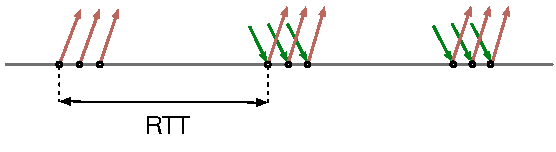
\includegraphics[width=0.4\textwidth]{arrival-cached}}\\
\subfigure[stable fresh data arrival, reflects publishing pattern]{\label{fig:fresh}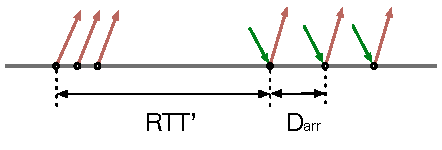
\includegraphics[width=0.35\textwidth]{arrival-fresh}}

\caption{Getting the latest data: arrival patterns for the cached and most recent data}
\label{fig:inter-arrival}
\end{figure}

During bootstrapping, the consumer "chases" the producer and aims to exhasut network cache of historical (non-real time) segments. By incerasing the number of outstanding interests, consumer "pulls cached data" out of the network unless the freshest data start to arrive. In order to control interest expresssion, a concept of $W$ (roughly an "interest window") is introduced (see Figure \ref{fig:w-concept}). Consumer expresses interests only when $W > 0$. At every moment, $W$ indicates how many outstanding interests can be sent out. Before the bootstrapping phase, consumer initializes $W$ with some value which reflects consumer's idea on how many interests are needed in order to exhaust network cache and reach the most recent data. 

\begin{figure}[t!]
\centering

\subfigure[$W$ concept]{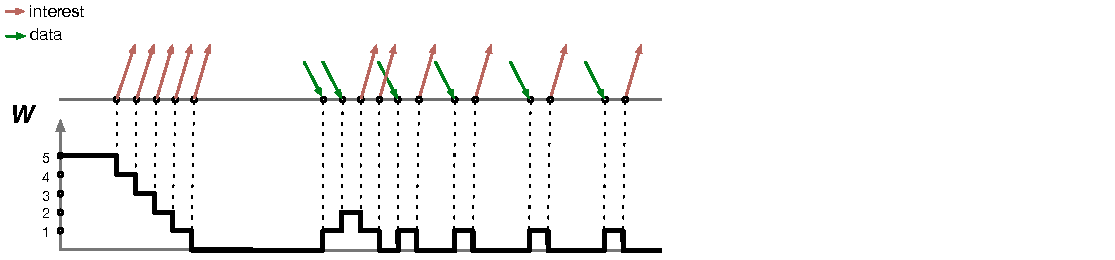
\includegraphics[width=0.35\textwidth]{w-concept}}
\subfigure[interests bursting ($W+3$)]{\label{fig:int-burst}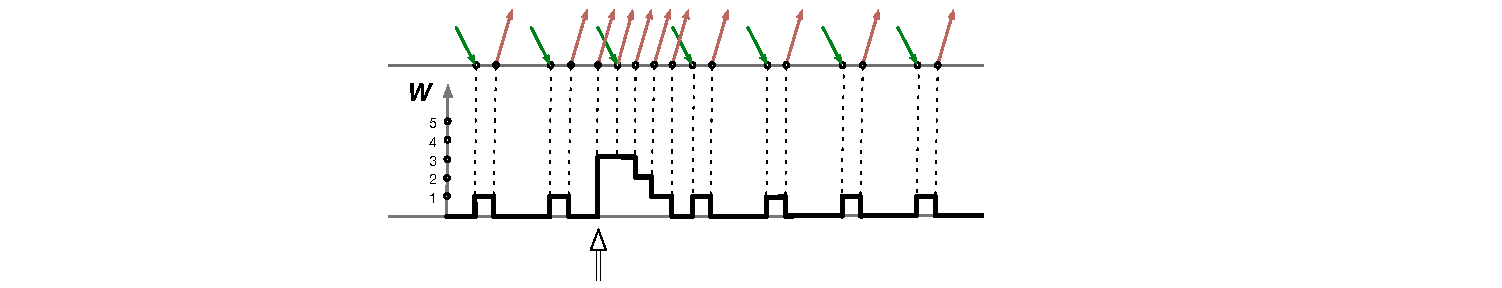
\includegraphics[width=0.35\textwidth]{int-burst}}
\subfigure[interests withholding ($W-3$)]{\label{fig:int-hold}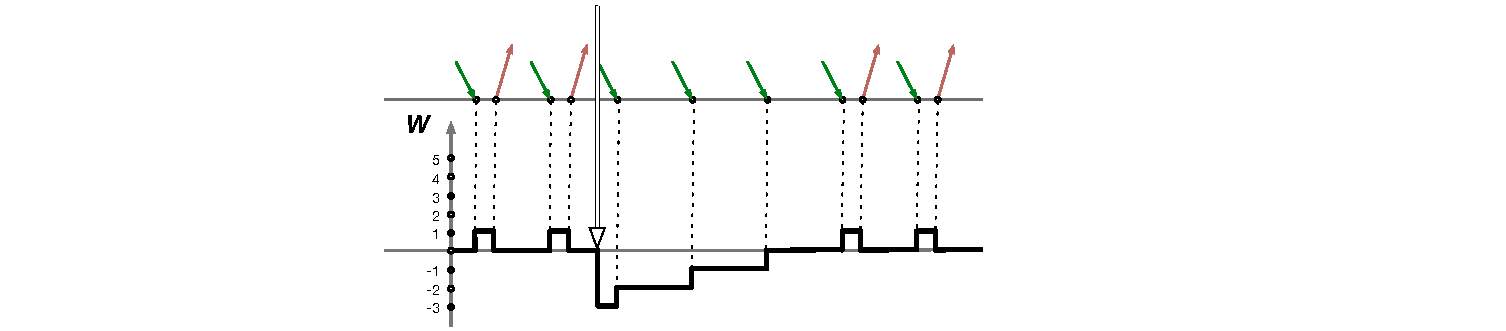
\includegraphics[width=0.35\textwidth]{int-hold}}

\caption{Managing interest expression}
\label{fig:w-concept}
\end{figure}


$W$ provides a simple mechanism which can be used to speed up or slow down interests expression. Any increase in $W$ value makes consumer to issue more interests (Figure \ref{fig:int-burst}), whereas decrease in $W$ holds consumer back from sending any new interests (Figure \ref{fig:int-hold}). Larger values of $W$ make consumer faster reach synchronized state with producer. However, larger value means larger number of outstanding interests and larger $RTT^\prime$ because of longer generation delays $d_{gen}$ for each media sample. By adjusting the value of $W$ and observing inter-arrival delays $D_{arr}$ consumer can find minimal $RTT^\prime$ value while still getting non-cached data, thus achieving best synchronization state with producer.

For more complex scenario of video streaming, consumer controls expression of "bulks" of interests instead of individual interests, because video frames are composed of several segments. In this case, $W$ is adjusted on per-frame basis, rather than per-segment. In all other respects, the same above logic can be applied.

Bootstrapping phase starts with issuing interest with enabled \textit{RightMostChild} selector in delta namespace for audio and key namespace for video. The reason, why this process differs for video streams is that consumer is not interested in fetching delta frames without having corresponding key frame for decoding. Once initial data segment of sample with number $S_{seed}$ has been received, consumer initializes $W$ with some initial value $N$ and asks for the next sample data $S_{seed}+1$ in the appropriate namespace. Upon receiveing first segments of sample $S_{seed}+1$, consumer initiates fetching process described above for all namespaces (delta and key, if available). Bootstrapping phase stops when consumer finds minimal value of $W$ which still allows receiving the most recent data - i.e. consumer reaches synchronized state with producer and switches to a normal fetching phase where no adjustments for $W$ are needed. 
% Listing \ref{lst:fetch-algo} shows pseudo-code for the bootstrapping phase.

% \begin{algorithm}
% \begin{algorithmic}

% \Function{Bootstrap}{Meta}

% \If {audio}
% 	\State $Nspc \gets DeltaNamespace$
% \Else
% 	\State $Nspc \gets KeyNamespace$
% \EndIf

% \State \Call{ExpressOne}{$RightMostChild$, $Nspc$}
% \Ensure Received data segment $Dseed$
% \State $Sseed \gets$\Call{GetSeqNumber}{$Dseed$}
% \State $NavgKey \gets$\Call{GetAvgSegNum}{$Meta$, $Key$}
% \State \Call{ExpressBulk}{$NavgKey$, $Sseed+1$, $Nspc$}
% \Ensure Received data segment $D$ for $Sseed+1$
% \State $J \gets$ \Call{GetDeltaNumber}{$D$}
% \State $NavgDelta \gets$\Call{GetAvgSegNum}{$Meta$, $Delta$}
% \State $DW \gets N$
% \State $W \gets DW$

% \While{$BootstrappingPhase$}

% \While{$W > 0$}
% 	\State \Call{ExpressBulk}{$NavgDelta$, $J$, $Delta$}
% 	\State $W \gets W-1$
% 	\State $J \gets J+1$
% \EndWhile

% \If {received segment $Dj$ for new sample}
% 	\State $W \gets W+1$
% \EndIf

% \EndWhile

% \State \Call{Switch}{$FetchingPhase$}

% \EndFunction

% \end{algorithmic}

% \label{lst:fetch-algo}
% \caption{Bootstrap}
% \end{algorithm}


%\subsubsection{Application-level PIT}
\textit{Application-level PIT} In most cases, consumers aim to express interests for the data not yet produced, so that they may be immediately satisfied when data is produced. The current NDN-CPP library provides a producer-side Memory Content Cache implementation into which data is published. However, it is only useful when data has been published and put in the cache before interest for this data has arrived. For the missing data, the interest is forwarded to producer application which has to store it in internal pending interests table (PIT) unless requested data is ready. This functionality seems quite common for low-latency applications has now been incorporated into the NDN-CPP library implementation.

\section{Implementation}
\label{sec:imp}
\ndnrtcName{} is implemented as a library written in C++, which is available at \url{https://github.com/remap/ndnrtc}. 
It provides publisher interface - for publishing arbitrary number of media streams (audio or video), and consumer interface with a callback for rendering decoded video frames in a host application. OS X platform is supported currently, though Linux build instructions will be added soon. 
The library distribution also comes with a simple console application which demonstrates the use of \ndnrtcName{} library.

\ndnrtcName{} exploits some functionality from several third-party libraries it is linked against with: NDN-CPP \cite{ndnccl} is used for NDN connectivity. The WebRTC framework \cite{webrtc} is utilized in two ways: 1) incorporation of the existing video codec; 2) full incorporation of the existing WebRTC audio pipeline, including echo cancellation;  3) OpenFec \cite{openfec} library is utilized for forwad error correction support.

Apart from the library, first desktop NDN videconferencing application \ndnconName{} \cite{ndncon} was implemented atop \ndnrtcName{}. It provides convenient UI for publishing and fetching media streams, text chat and organizing multi-party audio/video conferences.

\section{Evaluation}
\label{sec:eval} 

\subsection{Quality of experience} 

\subsection{Scaling}

\subsection{Performance of windowing}
\begin{figure}[t!]
\centering
%\captionsetup[subfigure]{aboveskip=-1pt,belowskip=-2pt}
\begin{scriptsize}
\subfigure[$W=10$: short chasing, larger $RTT^\prime$]{\def\svgwidth{0.48\textwidth}\input{w10.pdf_tex}}
\subfigure[$W=4$: longer chasing, smaller $RTT^\prime$]{\def\svgwidth{0.48\textwidth}\input{w4.pdf_tex}}
\subfigure[$W=3$: consumer can't exhasut cache, $RTT^\prime = RTT$]{\def\svgwidth{0.48\textwidth}\input{w3.pdf_tex}}
\end{scriptsize}
\caption{Larger $W$ decreases "chasing" phase, but increases $RTT^\prime$ for the same network configuration ($RTT\approx100ms$)}
\label{fig:ws}
\end{figure}

(Figure \ref{fig:ws} shows how bigger value of $W$ helps to exhaust cache faster). The number of outstanding interests is controlled by a consumer and directly influences how fast consumer can ``chase" the producer. Every time a new interest is expressed, $W$ gets decremented and when new data arrives, $W$ is incremented, thus allowing consumer to issue more interests.



\section{Conclusion and Future Work}
\label{sec:conclusion}


\begin{figure}[t!]
\centering
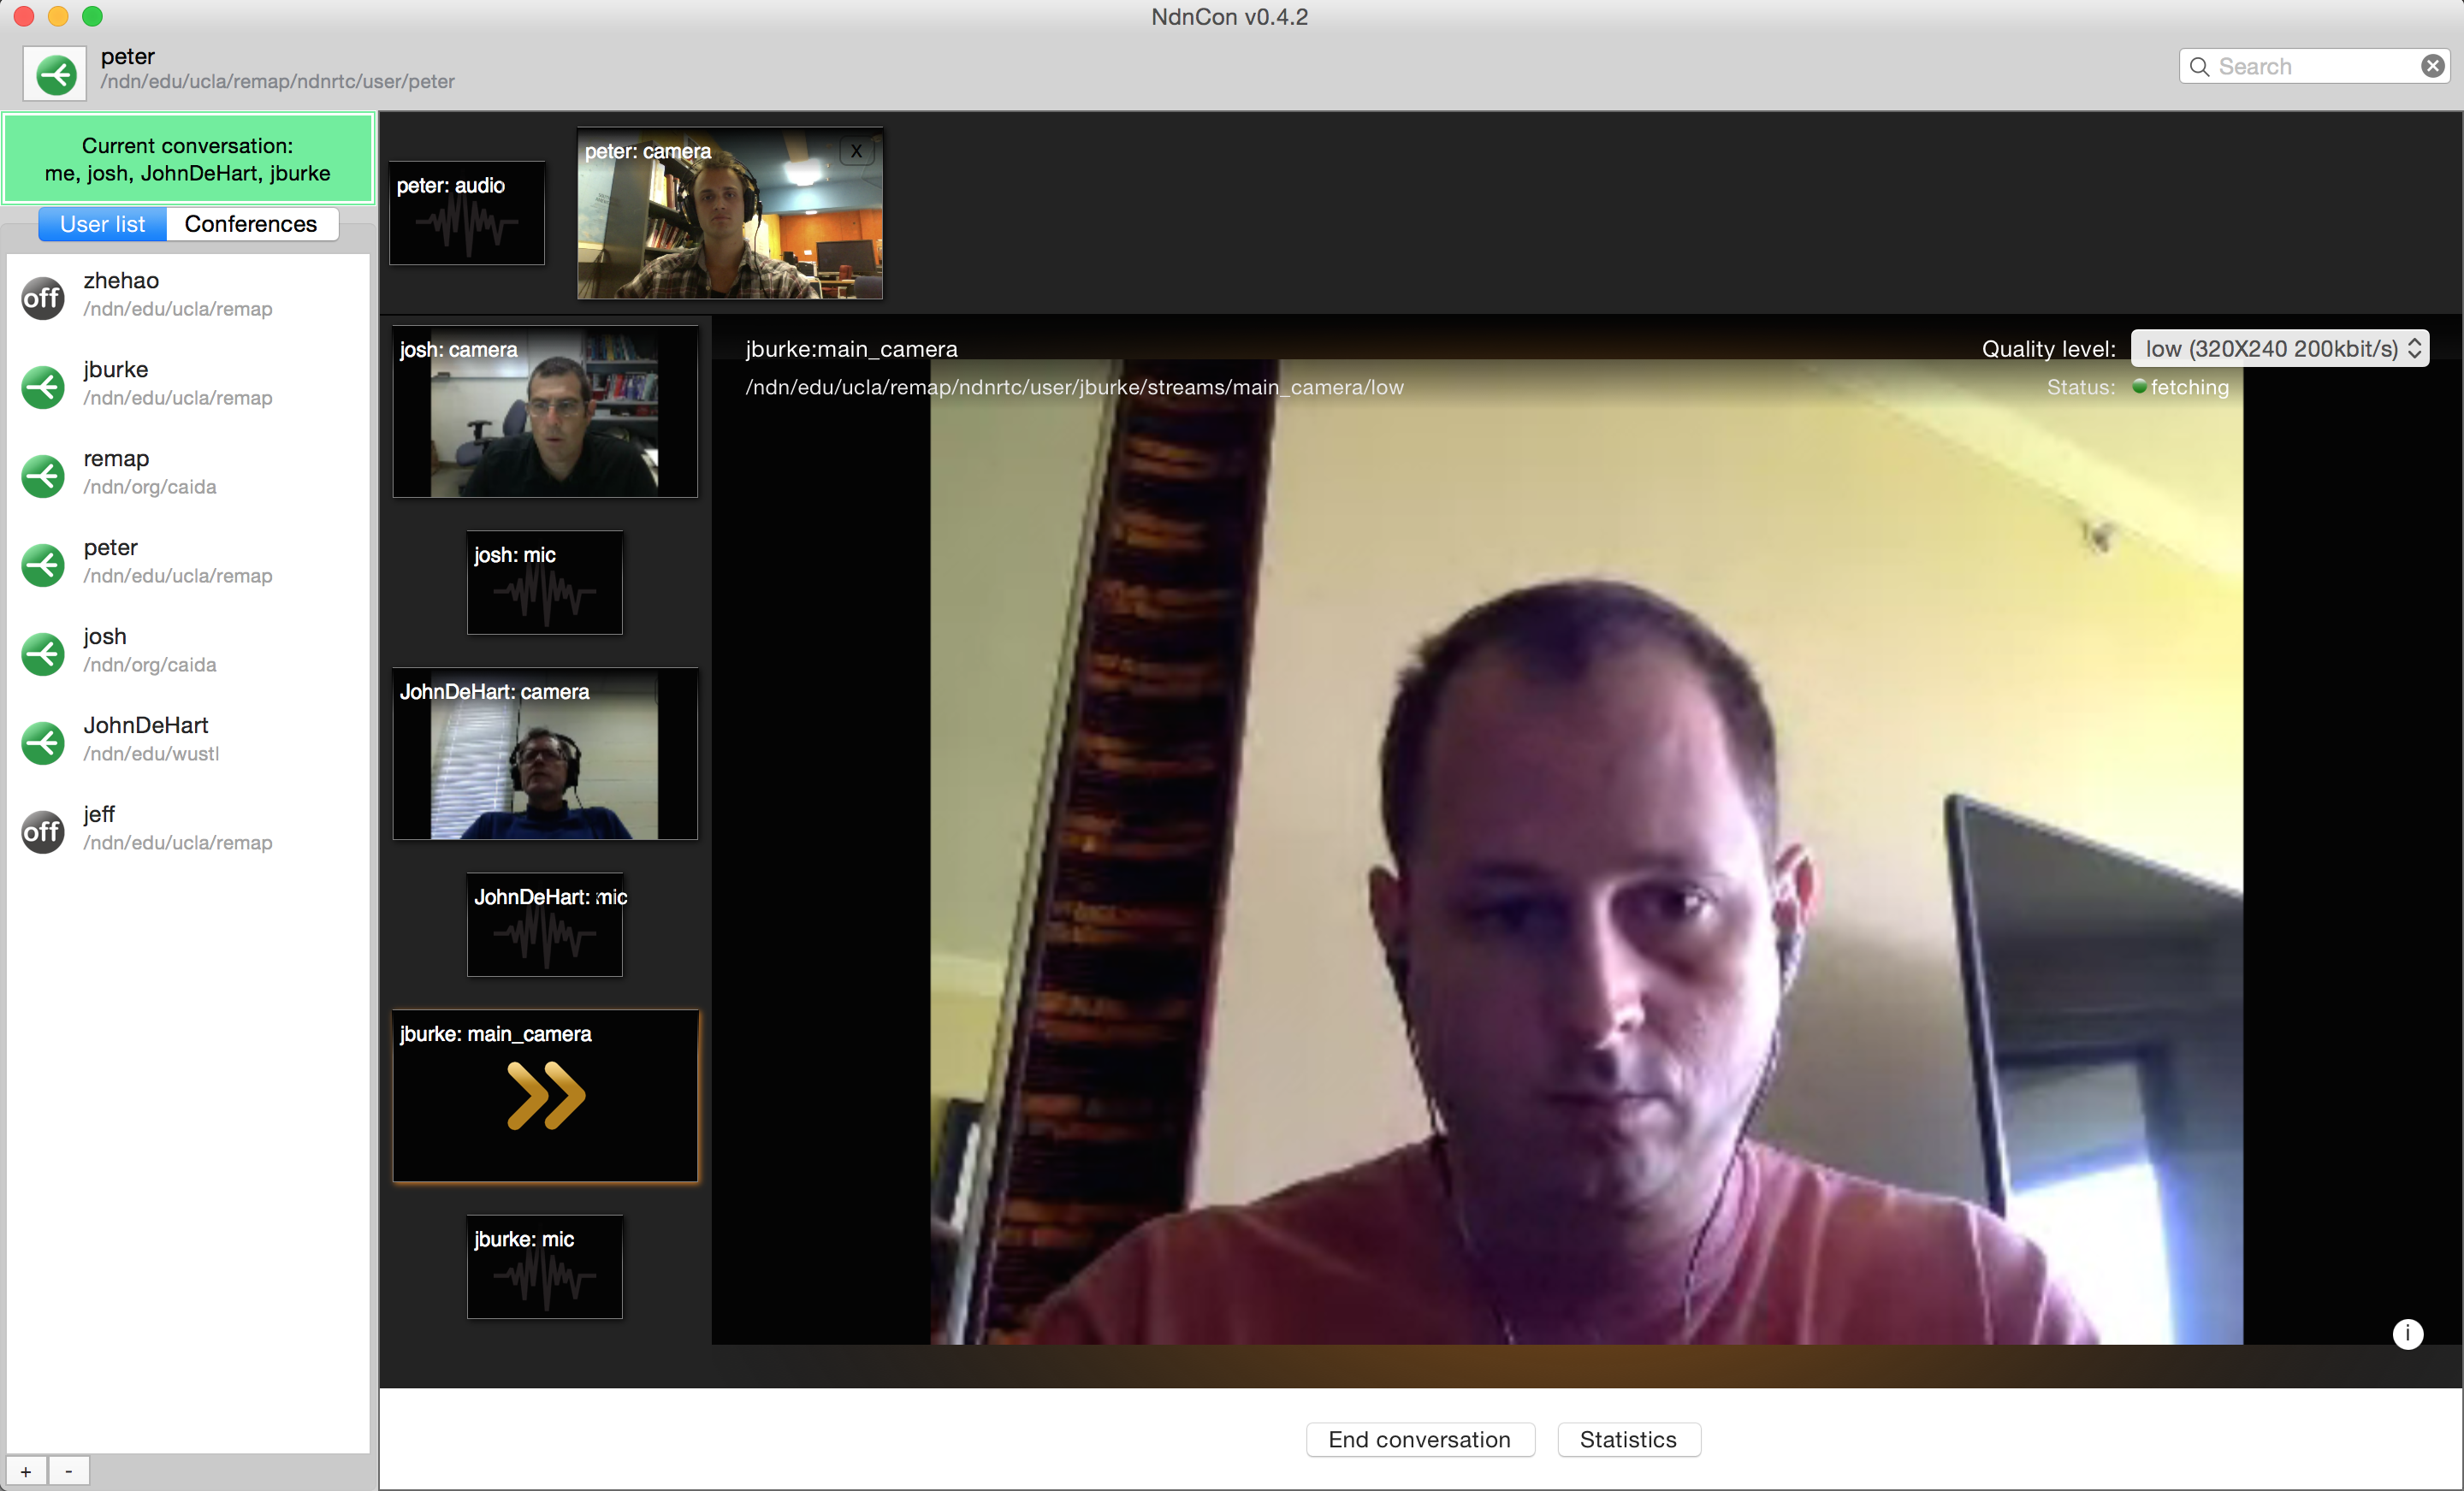
\includegraphics[width=0.3\textwidth]{ndncon}
\caption{\ndnconName{} screenshot [@@REPLACE]}
\label{fig:ndncon}
\end{figure}

%% TODO: Conclusion

Discuss quality of experience. 

Future work: 
\begin{itemize}[label={}]
\item \textbf{Adaptive rate control.} In current library design, producer may deliberately choose to publish several copies of the same video stream with different encoding parameters, thus allowing consumer to select the most appropriate stream for current network conditions. However, the selection is made manualy and depends on user's perceptual assessment of the retrieved media. Implementation of adaptive rate control would simplify this process and allow to utilize network more efficiently based on current conditions.

\item \textbf{Scalable video coding.} An elegant way to offload producer from publishing multiple copies of the same video stream in different bandwidths is to utilize Scalable Video Coding. By reflecting SVC layers in the namespace, consumer can have more freedom for adapting media streams to the current network. This opportunity should be explored and added in a future versions.

\item \textbf{Encryption-based access control} Current \ndnrtcName{} design supports basic content signing and verification. However, further basic security features are not yet implemented:, media data encryption, consumer access control.

\item \textbf{Conference management} 
Work on ndncon. unknown but verified publishers trust; 
\end{itemize}
%%signatures consistency checks for successive media packets 
%% need to add the above before publication %%;  


\section{Acknowledgements}
\label{sec:Acknowledgements}
This project was partially supported by the National Science Foundation (award CNS-1345318 and others) and a grant from Cisco.   The authors thank Lixia Zhang, Van Jacobson, and David Oran, as well as Eiichi Muramoto, Takahiro Yoneda, and Ryota Ohnishi from Panasonic Research, for their input and feedback. John DeHart, Josh Polterock, Jeff Thompson, and others on the NDN team provided invaluable testing of \ndnconName{}.  The initial forward error correction approach in \ndnrtcName{} was by Daisuke Ando. 

\bibliographystyle{abbrv}
\bibliography{bibliography}

\end{document}